% !TeX root = Jumppanen.tex
\title{Introduction to \pkg{BuildSys}: An R Package for Compiling and Debugging R Dynamic Libraries}
\author{by Paavo Jumppanen}

\maketitle

\abstract{%
A powerful feature of \strong{R} is the ability to make use of dynamically loaded libraries and call functions within (API) through the \code{.C} or \code{.CALL} interface. 
This allows the numerically intensive parts of an algorithm to be implemented in efficient compiled code (typically \strong{C/C++} or \strong{FORTRAN}) to  
obtain a significant boost in performance. The flip side of this approach is the complexity and difficulty of compilation, and in particular,
the debugging of the compiled code. \pkg{BuildSys} is a package that streamlines and integrates into \strong{R}, the process of both building and debugging
dynamically loaded libraries using well established and freely available tools and making debugging in particular, a more pleasant and 
productive part of the process.  
}

\hypertarget{introduction}{%
\subsection{Introduction}\label{introduction}}

The process of producing functionally correct dynamic libraries for \strong{R} can be broken down into three processes: (1) code compilation to produce object files,
(2) linking object files to produce a dynamically library and (3) runtime testing and debugging of the library code. In \strong{R} steps (1) and (2) 
are typically handled through the \samp{R CMD SHLIB}\citep{SHLIB} mechanism. Internally that mechanism typically relies on \dfn{GNU make}\citep{GnuMake} which 
in turn will typically use \dfn{GCC}\citep{gcc} (on most operating systems) or \dfn{CLANG/LLVM}\citep{LLVM} (on MacOS). On Windows based systems \dfn{GNU make} and \dfn{GCC}
are used and are made available by the \dfn{MINGW} based \dfn{Rtools} installation\citep{UsingRtools}. Compilation through \samp{R CMD SHLIB} 
involves the use of a generic makefile bundled within the \strong{R} installation that in turn uses environment variable string substitutions to specify the details 
of which files and compiler switches are needed. The command itself takes the command line and translates it into a suitable call to GNU make with the correct 
environment variables to obtain the desired compilation result. This is a simple, effective and portable way to handle compilation of shared 
libraries within \strong{R} packages, but for general use in circumstances where there are compile and/or link errors due to makefile mis-configuration 
(ie. missing include paths, library paths or libraries), it can be challenging to determine the source of the error in the command line specification. Furthermore, 
if the shared library contains many individual source files and uses of a number of static third party libraries, the required command line can become 
unwieldy and may also require the use of a secondary \emph{Makevars} file to specify addition compiler switches. For one off library development that is not targetting
packaging deployment but simply fulfilling a one off need, it can be easier to address the build issues in compiling a library by using a project specific makefile 
and \dfn{GNU make} invocation directly rather than going through the \samp{R CMD SHLIB} mechanism. \pkg{BuildSys} takes this approach by encapsulating a makefile within 
an S4 class that is managed from within \strong{R}. 

The third process in library development, debugging, is the most cumbersome part of currently used approaches and remains a stumbling 
block for many wishing to develop custom dynamic libraries, but who lack the knowledge and experience to make use of the available debugging 
tools to do so. The most commonly used debugger in an \strong{R} context is \dfn{GDB}\citep{GDB}, which provides realtime debugging of the dynamic library within the
host application (\strong{R}) via a large set of command line commands invoked at a command prompt in \dfn{GDB}. Similarly, debugging in \strong{R} on MacOS is performed using another 
command line based debugger, \dfn{LLDB}\citep{LLDB}. 

If users manage to build the library with appropriate debug information included, load the hosting \strong{R} session, have the debugger find and 
load the symbol table information and set active breakpoints, then they are part way to being able to successfully debug their library. However, 
one major issue remains that has to do with inspection of variables and other data structures. By default, both \dfn{GDB} and \dfn{LLDB} only 
know how to display intrinsic data types (bool, char, int, double etc.) in a meaningful way via their respective watch commands. To be able to 
display variables of a complex data type (structures or classes) they both must be provided with custom print code to visualise those complex 
data types. They both can display nominal information about complex data types but the default display of such types is non-intuitive, not particularly informative
and cumbersome to work with. This only magnifies in cases of indexing arrayed complex data types. It is this limitation that is the fundamental stumbling block for 
debugging code that leads to resorting to debugging via print statements rather than the employment of a debugger. 

If library developers only rely on native data types then this will not be an issue, however doing so implicitely requires the use of \code{.C} or 
\code{.CALL} mechanisms directly; see for instance \citep{DotC} and \citep{DotC2}. This in turn requires an intimate
knowledge of how \strong{R} natively represents data structures internally, which can be intimidating to the less experienced programmer. A more common approach is to 
use a C++ library that encapsulates the native \strong{R} data structures within complex data types, of which both \dfn{GDB} and \dfn{LLDB} are  
incapable of meaningfully visualising in their default state. 

The most widely used interface wrapper within the \strong{R} community is \pkg{Rcpp}\citep{RcppIntro},\citep{Rcpp}. Additionally, the packages \pkg{RcppEigen} 
and \pkg{TMB} build upon that interface to support \emph{linear algebra} \citep{RcppEigen}, \citep{RcppEigenLA}, \emph{automatic differentiation} \citep{TMBlaplace} and 
\emph{random effects models} \citep{TMB}. The utility of these packages alone represent a clear motivation for developing support for a more complete debugging 
experience. In fact, the initial motivation in developing \pkg{BuildSys} was to aid in debugging \pkg{TMB} based random effects model development in a 
\emph{fisheries MSE} (management strategy evaluation) context, although the package has general utility in any \strong{R} dynamic library development situation.

\hypertarget{exitising-debugging-approaches}{%
\subsection{Existing Debugging Approaches}
\label{exitising-debugging-approaches}}

Despite being widely used, documentation relating to \pkg{Rcpp} is notable for the lack of mention in any significant way of the process of debugging. For instance, the 
introductory paper \emph{Extending R with C++: A brief Introduction to Rcpp} \citep{RcppIntro} makes no mention of debugging, nor does the package documentation \citep{Rcpp}. 
This equally applies to packages that build upon \pkg{Rcpp}. Anecdotally, debugging appears to be the \emph{bain of existence} of an \strong{R} library developer and 
there appears to be ample need for simpler (but not at the expense of capability) approaches. \citep{DebuggingRandCcodeinR} advocates debugging using 
\dfn{GDB}\citep{GDB}, either through \dfn{EMACS} or \dfn{DDD}\citep{DDD} as a \dfn{GDB} front end, with memory errors being tackled with \dfn{valgrind}\citep{valgrind}. Similarly, 
\citep{DebuggingC_Cpp} advocates \dfn{GDB} or \dfn{LLDB} \citep{LLDB} (depending on the target operating system) for general debugging and \dfn{valgrind} for debugging memory 
errors, though makes the point that \emph{this is not for the faint of heart, and requires some C-level familiarity}. Although not explicit, this hints at the difficulty
many experience with debugging dynamic libraries for R. Although not specifically related to R, \citep{ImprovingCppDebug} laments the mis-givings of the debugging experience 
(circa 2020), summarises existing approaches and proposes the use of \dfn{Microsoft Visual Code}\citep{VSCodeDownload} as a possible solution. A common feature of the 
GUI front end debuggers is the need for a non-trivial setup stage. \dfn{Microsoft Visual Code} is no exception, although \pkg{BuildSys} includes processes that fully automate
this setup stage, thereby making the process of GUI hosted debugging of R dynamic libraries simpler and more accessible.

\hypertarget{visual-studio-code-extensions}{%
\subsection{GUI Debugging though Visual Studio Code}
\label{visual-studio-code-extensions}}

\dfn{Visual Studio Code} is a freely available and extensible cross platform text editor designed specifically for coding. It has been widely adopted in the general programming
community with a user base in excess of 2.6 million\citep{VCusers} and was \emph{the number one project in the 2017 GitHub Octoverse}. Central to the 
popularity of the editor is the ability to customize it to particular niche needs through downloadable extensions. Of note in this particular application of \dfn{Visual Studio Code} 
is the \emph{Microsoft C/C++ extension} \citep{VSCodeCCppExt} which, apart from providing editor feature support targeting the C and C++ languages, also provides support for 
debugging via the machine interface to \dfn{GDB} (\dfn{GDB-MI}). It also provided debugging support on \dfn{MacOS} via \dfn{LLDB-MI}, however Apple have since abandoned support for \dfn{LLDB-MI} making 
the debugging support via this extension on MacOS inopperable. However, a third party extension, \dfn{CodeLLDB}\citep{CodeLLDB}, provides the equivalent debugging support that does not rely on
\dfn{LLDB-MI} to interface with \dfn{LLDB} and works with current versions of \dfn{MacOS}. 

Both \emph{CodeLLDB} and the \emph{Microsoft C/C++ extension} make debugging available through added configurations. These are codified using \dfn{JSON}\citep{JSON} format configration files;
one to specify how to launch or attach a debug session (the \emph{launch.json} file) and one to specify information needed to be able to correctly interpret the code within the debugging 
session (the \emph{c\_cpp\_properties.json} file). Typical \emph{launch.json} and \emph{c\_cpp\_properties.json} files are illustrated in Figures \ref{fig:launchJSON} and \ref{fig:CnCppProp}.
Whilst not overly complex, it is relatively easy to mis-configure and be left with partially operable or completely broken debugging. In the case of \pkg{BuildSys} these two files are 
automatically generated for the user and placed in the necessary folder so no user intervention is required and debugging works as expected.

\begin{Schunk}
  \begin{figure}[htbp]
  {\centering}
  \begin{verbatim}
  {
    "version": "0.2.0",
    "configurations": [
      {
        "name": "(gdb) Launch",
        "type": "cppdbg",
        "request": "launch",
        "targetArchitecture":"x86_64",
        "program": "C:/Users/jum002/DOCUME~1/R/R-40~1.5/bin/x64/Rgui.exe",
        "args": ["--no-save", "--no-restore"],
        "stopAtEntry": false,
        "cwd": "C:/Users/jum002/DOCUME~1/Test/CONVOL~1.RPR",
        "environment": [{"name":"R_HOME",
                         "value":"C:/Users/jum002/Documents/R/R-4.0.5"}],
        "externalConsole": true,
        "MIMode": "gdb",
        "miDebuggerPath": "C:/rtools40/mingw64/bin/gdb.exe",
        "miDebuggerArgs": "--init-command debugCmd.txt",
        "setupCommands": [
          {
            "description": "Enable pretty-printing for gdb",
            "text": "-enable-pretty-printing",
            "ignoreFailures": true
          }
        ]
      }
    ]
  }
  \end{verbatim}
  \caption[A Typical launch.json File]{A Typical launch.json File}
  \label{fig:launchJSON}
  \end{figure}
\end{Schunk}
    
\begin{Schunk}
  \begin{figure}[htbp]
  {\centering}
  \begin{verbatim}
  {
    "configurations": [
    {
      "name": "Win32",
      "intelliSenseMode": "gcc-x64",
      "includePath": ["${workspaceFolder}",
                      "C:/rtools40/mingw64/include/**",
                      "C:/rtools40/usr/include/**",
                      "C:/Users/jum002/DOCUME~1/R/R-40~1.5/include/**",
                      "C:/Users/jum002/DOCUME~1/Test/**",
                      "C:/Users/jum002/DOCUME~1/R/R-40~1.5/include/**"],
      "defines": [],
      "compilerPath": "C:/rtools40/mingw64/bin/gcc.exe",
      "cStandard": "c89",
      "cppStandard": "c++14",
      "browse": {
          "limitSymbolsToIncludedHeaders": true,
          "databaseFilename": ""
        }
      }
    ],
    "version": 4
  }
  \end{verbatim}
  \caption[A Typical c\_cpp\_properties.json File]{A Typical c\_cpp\_properties.json File}
  \label{fig:CnCppProp}
  \end{figure}
\end{Schunk}
    
Within a \emph{Visual Code} debug session (Figure \ref{fig:VisualCode}) the user has the ability to:

\begin{itemize}
\item set breakpoints either with or without conditions (ie. breakpoint counts and breakpoints triggered by data expression)
\item control execution flow with, single stepping, stepping in and stepping out
\item add variable watches to the watch window
\item see contexual local variable data
\item see the stack frame and navigate through the call trace
\end{itemize}

Of particular note is the ability to use complex evaluated expressions that update with program flow within the watch window (\code{xa[i]}, \code{xb[j]} in Figure \ref{fig:VisualCode}). 
Whilst a seasoned \dfn{GDB} or \dfn{LLDB} user could extract this information in the command line equivalent, multiple commands taken from a vast command set are typically required,
making this approach challenging for a novice user of these products. On the other hand, in a GUI presented interface the process of utilising these debugging features is made obvious, 
requires little understanding of the debugger command set, and presents the information in a readily digestible manner, making the debugging experience less daungting and more productive, 
particularly for the novice user. 

\begin{Schunk}
  \begin{figure}[htbp]
  {\centering 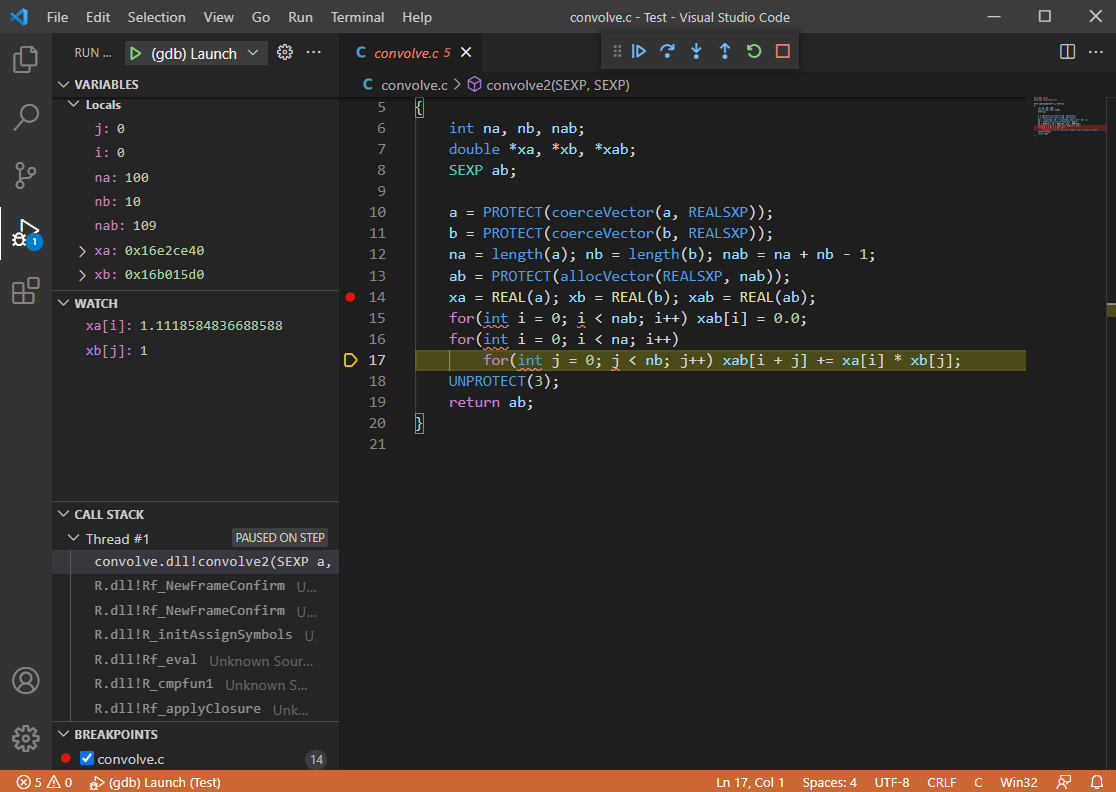
\includegraphics[width=0.95\textwidth]{VisualCode} 

  }
  \caption[Visual Code Debug Session]{Visual Code Debug Session}\label{fig:VisualCode}
  \end{figure}
\end{Schunk}
  

\hypertarget{BuildSys-Overview}{%
\subsection{An Overview in Using BuildSys}
\label{visual-studio-code-extensions}}

A useful illustration of BuildSys is applying it to the code examples given in \emph{Extending R with C++: A Brief Introduction to Rcpp}\citep{RcppIntro}. The main example is 
the convolve .CALL one first appearing in \emph{Writing R Extensions}\citep{Rextensions} Manual. Assume the code given below is in the file \emph{"convolve.c"} in the folder \emph{"\textasciitilde/ConvoleRext"}.

\begin{Schunk}
  \begin{Sinput}
  #include <R.h>
  #include <Rinternals.h>
  
  SEXP convolve2(SEXP a, SEXP b)
  {
      int na, nb, nab;
      double *xa, *xb, *xab;
      SEXP ab;
  
      a = PROTECT(coerceVector(a, REALSXP));
      b = PROTECT(coerceVector(b, REALSXP));
      na = length(a); nb = length(b); nab = na + nb - 1;
      ab = PROTECT(allocVector(REALSXP, nab));
      xa = REAL(a); xb = REAL(b); xab = REAL(ab);
      for(int i = 0; i < nab; i++) xab[i] = 0.0;
      for(int i = 0; i < na; i++)
          for(int j = 0; j < nb; j++) xab[i + j] += xa[i] * xb[j];
      UNPROTECT(3);
      return ab;
  }
  \end{Sinput}
\end{Schunk}

To create a BuildSys project, compile this file into a dynamic library and load it run,

\begin{Schunk}
  \begin{Sinput}
  library(BuildSys)
  Project <- new("BSysProject", WorkingFolder="~/ConvolveRext", Name="ConvolveRext")
  make(Project)
  loadLibrary(Project)
  \end{Sinput}
\end{Schunk}

in and R session. To execute the example use,

\begin{Schunk}
  \begin{Sinput}
  conv <- function(a, b) .Call("convolve2", a, b)
  a <- rnorm(100)
  b <- rep(1.0, times=10)
  conv(a, b)
  \end{Sinput}
\end{Schunk}

giving the output,

\begin{Schunk}
  \begin{Sinput}
  [1]  0.98293848  1.24876911  0.60384865  1.55706527  0.69375036  2.56200291
  [7]  3.35339771  1.99702141  0.36106970  1.05994411 -0.68884999 -1.44729536
   .
   .
   .
 103]  2.32572624  2.79692698  2.37123793  1.45493333  1.62681502  0.25344351
[109]  0.08219538
  \end{Sinput}
\end{Schunk}

Note that by default, the \code{make()} command in \pkg{BuildSys} will build code with no optimisations and full debug information. 
Constructing a release build with full optimisation can be achieved by supplying the \code{Debug=FALSE} argument when creating the project. 

To debug the code in an interactive GUI session call execute \code{vcDebug(Project)} in R. This assumes that
\emph{Visual Studio Code} and the necessary extensions are correctly installed as per the package requirements, the process of which is discussed in 
detail in the package help (\code{{?BuildSys}} at an R command prompt). On executing \code{vcDebug(Project)}, R will spawn \emph{Visual Studio Code} 
with the correct \emph{JSON} files to debug the dynamic library. Within \emph{Visual Studio Code} open the file \emph{"convolve.c"}, set any required
breakpoints and then press the \emph{F5} key to start a debug session. \emph{Visual Studio Code} will then spawn a new session of R whose initial state
will be the same as the state of the parent R session when \code{vcDebug(Project)} was called. This behaviour is implemented as a aid to debugging as most 
debugging sessions will require R based test harmess code / data to debug with and by choosing to execute \code{vcDebug(Project)} after the R test harness is 
set up we no longer need to do it in the debugging session, irrespective of how many times we re-start debugging the dynamic library. In our case 
the test data was already in place and the library loaded prior to calling \code{vcDebug(Project)} so in our debugging session all we need to run is \code{conv(a, b)}. 
The execution then drops out into the debug session at our set breakpoint as in Figure \ref{fig:VisualCode}. Note that variable watches can be valid C/C++
expressions provided they do not involve function calls. Thus the variables being updated in the loop can be watched with the watch expressions, \code{xa[i]}, 
\code{xb[j]} and \code{xab[i+j]} and they will be updated as and when the data changes. 

Now turning to the \emph{Rcpp} re-implementation of this example, assume the code given below is in the file \emph{"convolve.cpp"} in the folder \emph{"\textasciitilde/ConvoleRcpp"}.

\begin{Schunk}
  \begin{Sinput}
  #include "Rcpp.h"

  using namespace Rcpp;
  
  NumericVector convolve2(const NumericVector& a, 
                          const NumericVector& b)
  {
      int i, j;
      int na = a.size();
      int nb = b.size();
      int nab = na + nb - 1;
  
      NumericVector ab(nab);
  
      for (i = 0 ; i < na ; i++)
      {
          for (j = 0 ; j < nb ; j++)
          {
              ab[i + j] += a[i] * b[j];
          }
      }
  
      return ab;
  }
  
  // Dynamic lib entry point code
  RcppExport SEXP convolveCpp(SEXP aSEXP, SEXP bSEXP)
  {
      Rcpp::RObject rcpp_result_gen;
      Rcpp::RNGScope rcpp_rngScope_gen;
      Rcpp::traits::input_parameter< const NumericVector& >::type a(aSEXP);
      Rcpp::traits::input_parameter< const NumericVector& >::type b(bSEXP);
      rcpp_result_gen = Rcpp::wrap(convolve2(a, b));
      return rcpp_result_gen;
  }
  \end{Sinput}
\end{Schunk}

Note that unlike the original example, this version includes the explicit entry point function \code{convolveCpp()}. 
Normally code in \pkg{Rcpp} is built using the R functions \code{cppFunction()} and \code{sourceCpp()}. These functions 
transparently take the C++ code, copy it to a duplicate source code file, then add wrapper functions for the C++ functions 
marked with \code{Rcpp\:\:Export} and the compiles that extended source file to produce the necessary dynamic library. As we are 
not using the normal \pkg{Rcpp} compilation route the wrapper code needs to be hand written. 
Similarly to create a BuildSys project, compile this file into a dynamic library and load it run,

\begin{Schunk}
  \begin{Sinput}
  library(BuildSys)
  library(Rcpp)
  Project <- new("BSysProject", WorkingFolder="~/ConvolveRcpp", Name="ConvolveRcpp")
  make(Project)
  loadLibrary(Project)
  \end{Sinput}
\end{Schunk}

in and R session and to execute the example use,

\begin{Schunk}
  \begin{Sinput}
  conv <- function(a, b) .Call("convolveCpp", a, b)
  a <- rnorm(100)
  b <- rep(1.0, times=10)
  conv(a, b)
  \end{Sinput}
\end{Schunk}

giving the identical output to the previous example. As with the C version of convolve, variable watches of 
array elements is also possible. However, in this case we require more complex expressions to do so as the 
arrays are implemented as C++ classes rather than intrinsic C arrays. The corresponding expressions in this
case are \code{((a).cache).start[i]}, \code{((b).cache).start[j]} and \code{(((ab).cache).start)[i+j]} as 
shown in Figure \ref{fig:RcppDebug}.

\begin{Schunk}
  \begin{figure}[htbp]
  {\centering 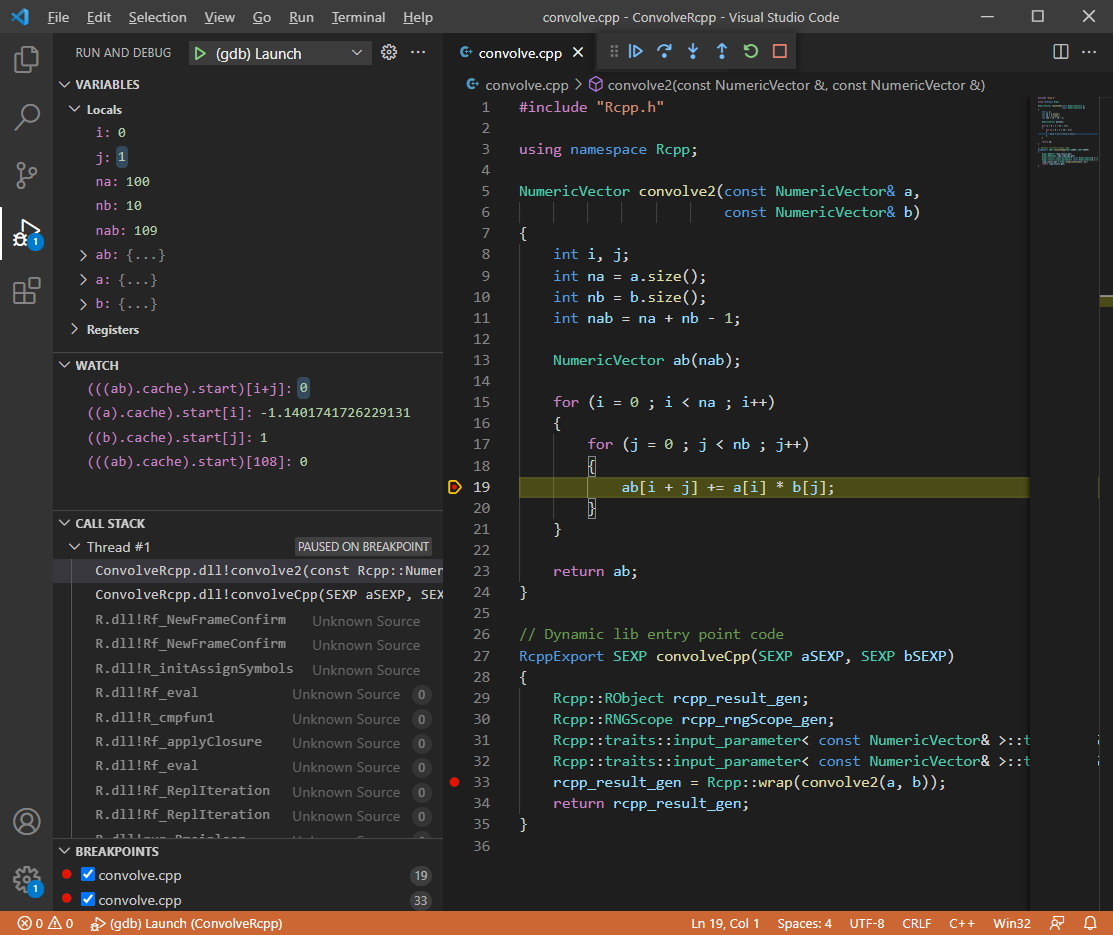
\includegraphics[width=0.95\textwidth]{RcppDebug} 

  }
  \caption[Debugging Rcpp Code]{Debugging Rcpp Code}\label{fig:RcppDebug}
  \end{figure}
\end{Schunk}

Similarly, a useful illustration of BuildSys applied to TMB is made by applying it to the code example given 
in \emph{TMB: Automatic Differentiation and Laplace Approximation}\citep{TMBlaplace}. The code in question is 
an implementation of the \emph{theta logistic population model} of \citep{WangG} and \citep{PedersenEtAl}.
Assume the C++ source code given below is in the file \emph{"thetalog.cpp"} in the folder \emph{"\textasciitilde/thetalog"}. 
To illustrate bounds checking the code also includes a coding error in the loops that will index beyond the array boundaries.

\begin{Schunk}
  \begin{Sinput}
    // Theta logistic population model from Pedersen et al 2012, Ecol. Modelling.
    #include <TMB.hpp>
    template<class Type>
    Type objective_function<Type>::operator() ()
    {
      /* Data section */
      DATA_VECTOR(Y);

      /* Parameter section */
      PARAMETER_VECTOR(X);
      PARAMETER(logr0);
      PARAMETER(logtheta);
      PARAMETER(logK);
      PARAMETER(logQ);
      PARAMETER(logR);

      /* Procedure section */
      Type r0       = exp(logr0);
      Type theta    = exp(logtheta);
      Type K        = exp(logK);
      Type Q        = exp(logQ);
      Type R        = exp(logR);
      int timeSteps = Y.size();
      Type ans      = 0;

      for (int i = 1 ; i <= timeSteps ; i++)
      {
        Type m = X[i - 1] + r0 * (1.0 - pow(exp(X[i - 1]) / K, theta));
        ans -= dnorm(X[i], m, sqrt(Q), true);
      }

      for (int i = 0 ; i <= timeSteps ; i++)
      {
        ans -= dnorm(Y[i], X[i], sqrt(R), true);
      }

      return ans;
    }
  \end{Sinput}
\end{Schunk}

The R code required to compile the C++ code and be readied for debugging is given by,

\begin{Schunk}
  \begin{verbatim}
  library(BuildSys)
  library(TMB)
  Project <- new("BSysProject", WorkingFolder="~/thetalog", Name="thetalog")
  make(Project)
  loadLibrary(Project)
  y <- scan("thetalog.dat", skip = 3, quiet = TRUE)
  loadLibrary(Project)
  data       <- list(y = y)
  parameters <- list(u      = data$y * 0,
                     logr0  = 0,
                     logpsi = 0,
                     logK   = 6,
                     logQ   = 0,
                     logR   = 0)

  vcDebug(Project)
  \end{verbatim}
\end{Schunk}

To debug we set a breakpoint on a part of code prior to the loop (say \code{DATA\_VECTOR(Y);}) and commence 
the debug session in Visual Studio Code by pressing the \emph{F5} key and running the following R code 
in the spawned R session,

\begin{Schunk}
  \begin{Sinput}
    obj <- MakeADFun(data, parameters, random = "u", DLL = "thetalog")
  \end{Sinput}
\end{Schunk}

The reason for adding the initial breakpoint is due to a limitation in (at least in the Windows version) Visual Studio Code not 
being able to activate a configuration defined breakpoint on startup. When debugging \pkg{TMB} code \pkg{BuildSys} adds the file \emph{bsys\_abort.cpp}
to the project. This file implements a C standard library override to the \code{abort()} function which TMB calls in response to 
boundary errors in indexing. The \emph{launch.json} file includes startup commands for the debugger to set a breakpoint on the call to 
the \emph{bsys\_abort.cpp} function but if we fail to interrupt the debug session with the added entry point breakpoint to our TMB code, this 
abort handler breakpoint is never properly activated. Until this issue is resolved this is a suitable work around. 

Having execution halt at our breakpoint line (\code{DATA\_VECTOR(Y);}), continuing exection results in the code execution halting in the \code{abort()}
function because of the introduced boundary error. 

Discuss stuff to do with array bounds exceptions.

\hypertarget{Conclusions}{%
\subsection{Conclusions}
\label{Conclusions}}

Discuss conclusions.

\bibliography{BuildSysReferences.bib}

\address{%
Paavo Jumppanen\\
CSIRO Marine and Atmospheric Research\\%
Castray Esplanade,\\Battery Point TAS 7004,\\Australia\\
%
\url{https://www.csiro.au}%
\\\href{mailto:paavo.jumppanen@csiro.au}{\nolinkurl{paavo.jumppanen@csiro.au}}
}
